% !TeX program = pdfLaTeX
\documentclass[12pt]{article}
\usepackage{amsmath}
\usepackage{graphicx,psfrag,epsf}
\usepackage{enumerate}
\usepackage{natbib}
\usepackage{textcomp}
\usepackage[hyphens]{url} % not crucial - just used below for the URL
\usepackage{hyperref}
\providecommand{\tightlist}{%
  \setlength{\itemsep}{0pt}\setlength{\parskip}{0pt}}

%\pdfminorversion=4
% NOTE: To produce blinded version, replace "0" with "1" below.
\newcommand{\blind}{0}

% DON'T change margins - should be 1 inch all around.
\addtolength{\oddsidemargin}{-.5in}%
\addtolength{\evensidemargin}{-.5in}%
\addtolength{\textwidth}{1in}%
\addtolength{\textheight}{1.3in}%
\addtolength{\topmargin}{-.8in}%

%% load any required packages here


\usepackage{color}
\usepackage{fancyvrb}
\newcommand{\VerbBar}{|}
\newcommand{\VERB}{\Verb[commandchars=\\\{\}]}
\DefineVerbatimEnvironment{Highlighting}{Verbatim}{commandchars=\\\{\}}
% Add ',fontsize=\small' for more characters per line
\usepackage{framed}
\definecolor{shadecolor}{RGB}{248,248,248}
\newenvironment{Shaded}{\begin{snugshade}}{\end{snugshade}}
\newcommand{\AlertTok}[1]{\textcolor[rgb]{0.94,0.16,0.16}{#1}}
\newcommand{\AnnotationTok}[1]{\textcolor[rgb]{0.56,0.35,0.01}{\textbf{\textit{#1}}}}
\newcommand{\AttributeTok}[1]{\textcolor[rgb]{0.77,0.63,0.00}{#1}}
\newcommand{\BaseNTok}[1]{\textcolor[rgb]{0.00,0.00,0.81}{#1}}
\newcommand{\BuiltInTok}[1]{#1}
\newcommand{\CharTok}[1]{\textcolor[rgb]{0.31,0.60,0.02}{#1}}
\newcommand{\CommentTok}[1]{\textcolor[rgb]{0.56,0.35,0.01}{\textit{#1}}}
\newcommand{\CommentVarTok}[1]{\textcolor[rgb]{0.56,0.35,0.01}{\textbf{\textit{#1}}}}
\newcommand{\ConstantTok}[1]{\textcolor[rgb]{0.00,0.00,0.00}{#1}}
\newcommand{\ControlFlowTok}[1]{\textcolor[rgb]{0.13,0.29,0.53}{\textbf{#1}}}
\newcommand{\DataTypeTok}[1]{\textcolor[rgb]{0.13,0.29,0.53}{#1}}
\newcommand{\DecValTok}[1]{\textcolor[rgb]{0.00,0.00,0.81}{#1}}
\newcommand{\DocumentationTok}[1]{\textcolor[rgb]{0.56,0.35,0.01}{\textbf{\textit{#1}}}}
\newcommand{\ErrorTok}[1]{\textcolor[rgb]{0.64,0.00,0.00}{\textbf{#1}}}
\newcommand{\ExtensionTok}[1]{#1}
\newcommand{\FloatTok}[1]{\textcolor[rgb]{0.00,0.00,0.81}{#1}}
\newcommand{\FunctionTok}[1]{\textcolor[rgb]{0.00,0.00,0.00}{#1}}
\newcommand{\ImportTok}[1]{#1}
\newcommand{\InformationTok}[1]{\textcolor[rgb]{0.56,0.35,0.01}{\textbf{\textit{#1}}}}
\newcommand{\KeywordTok}[1]{\textcolor[rgb]{0.13,0.29,0.53}{\textbf{#1}}}
\newcommand{\NormalTok}[1]{#1}
\newcommand{\OperatorTok}[1]{\textcolor[rgb]{0.81,0.36,0.00}{\textbf{#1}}}
\newcommand{\OtherTok}[1]{\textcolor[rgb]{0.56,0.35,0.01}{#1}}
\newcommand{\PreprocessorTok}[1]{\textcolor[rgb]{0.56,0.35,0.01}{\textit{#1}}}
\newcommand{\RegionMarkerTok}[1]{#1}
\newcommand{\SpecialCharTok}[1]{\textcolor[rgb]{0.00,0.00,0.00}{#1}}
\newcommand{\SpecialStringTok}[1]{\textcolor[rgb]{0.31,0.60,0.02}{#1}}
\newcommand{\StringTok}[1]{\textcolor[rgb]{0.31,0.60,0.02}{#1}}
\newcommand{\VariableTok}[1]{\textcolor[rgb]{0.00,0.00,0.00}{#1}}
\newcommand{\VerbatimStringTok}[1]{\textcolor[rgb]{0.31,0.60,0.02}{#1}}
\newcommand{\WarningTok}[1]{\textcolor[rgb]{0.56,0.35,0.01}{\textbf{\textit{#1}}}}



\begin{document}


\def\spacingset#1{\renewcommand{\baselinestretch}%
{#1}\small\normalsize} \spacingset{1}


%%%%%%%%%%%%%%%%%%%%%%%%%%%%%%%%%%%%%%%%%%%%%%%%%%%%%%%%%%%%%%%%%%%%%%%%%%%%%%

\if0\blind
{
  \title{\bf Extending ggplot2 statistical geometries}

  \author{
        Evangeline Reynolds \thanks{The authors gratefully acknowledge \ldots{}} \\
    Dean Data Cell, West Point\\
     and \\     Author 2 \\
    Department of ZZZ, University of WWW\\
      }
  \maketitle
} \fi

\if1\blind
{
  \bigskip
  \bigskip
  \bigskip
  \begin{center}
    {\LARGE\bf Extending ggplot2 statistical geometries}
  \end{center}
  \medskip
} \fi

\bigskip
\begin{abstract}
Ggplot2, the implementation of the grammar of graphics in the R
statistical programming language, is a popular open source project. The
package's interface lets creators separate data visualization concerns
--- including declaration of data, variable representations by visual
channels, determination of coordinate systems, selection of geometric
shapes taking on the aesthetic representation --- which means users have
great freedom in the creation and customization of charts. Ggplot2 comes
with a large number of geometric shapes that can represent variables in
data sets. Some of these shapes are drawn after statistical
transformation, such as boxplots, linear regressions, or histograms. But
many statistical concepts do not have easy-to-use geometries for
representing statistical summaries. This paper presents a new extension
package \texttt{ggxmean}, that include new \texttt{geoms} useful for
easily visualizing an important set of additional statistical concepts.
\end{abstract}

\noindent%
{\it Keywords:} 3 to 6 keywords, that do not appear in the title
\vfill

\newpage
\spacingset{1.45} % DON'T change the spacing!

\hypertarget{introduction}{%
\section{Introduction}\label{introduction}}

The grammar of graphics framework, proposed by Leland Wilkinson in 1999,
that identified `seven orthogonal components' in the creation of data
visualizations.\\
Wilkinson asserted that if data visualization packages were created
using a separation of concerns approach -- dividing decision making
surrounding these components --- the packages would be able to ``draw
every statistical graphic''. The grammar of graphic principles were
incredibly powerful and gave rise to a number of visualization platforms
including Tableau, vega-lite, and ggplot2.

Statistical educators that introduce students to one of these tools
arguably are doing more than constructing one-off plots to discuss
statistical principles with students: they are introducing students to
`a powerful way of thinking about data visualization'.

Statistical educators often use ggplot2 as their
grammar-of-graphics-based data visualization tool as students can learn
it along side the rich statistical ecosystem of the R programming
language. The R programming language thus may serve as a one-stop-shop
for statistical tooling; with recent developments in packages and IDEs
writing code is becoming more accessible and welcoming to newcomers.

Still, using ggplot2 for statistical education can be a challenge. When
it is used to discuss statistical concepts, the plotting task can
sometime scatter the focus on statistical concepts.

\hypertarget{the-status-quo-adding-the-mean}{%
\subsection{The status quo: adding the
mean}\label{the-status-quo-adding-the-mean}}

Consider for example, a the seemingly simple enterprise of adding a
vertical line at the mean of x, perhaps atop a histogram or density
plot.

\begin{center}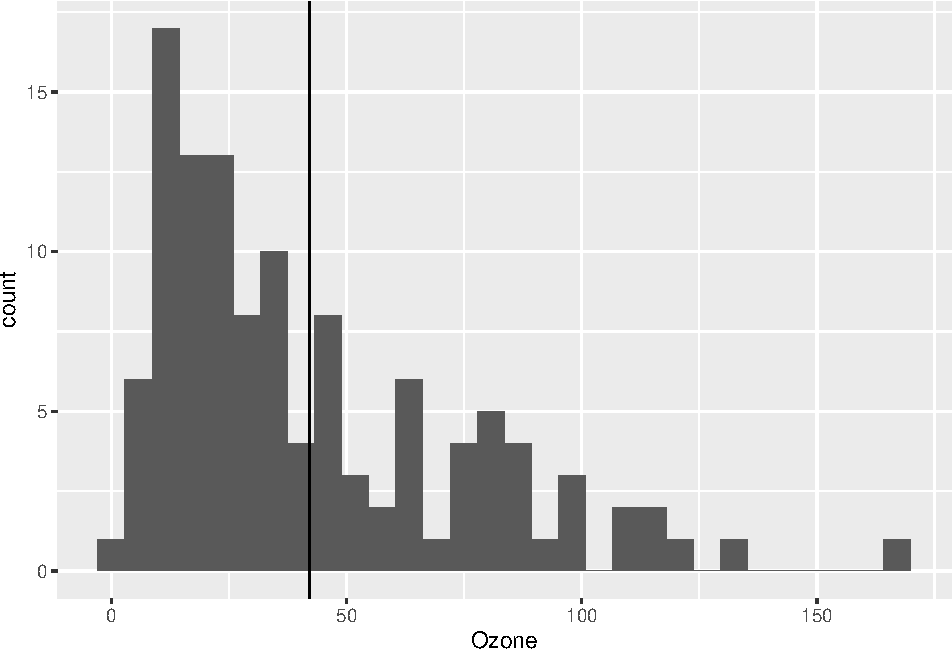
\includegraphics[width=0.5\linewidth]{manuscript_files/figure-latex/unnamed-chunk-2-1} \end{center}

Creating this plot requires greater focus on ggplot2 \emph{syntax},
likely detracting from discussion of \emph{the mean} that statistical
instructors desire.

The status quo syntax is as follows:

\begin{Shaded}
\begin{Highlighting}[]
\KeywordTok{library}\NormalTok{(tidyverse)}
\KeywordTok{library}\NormalTok{(magrittr)}

\KeywordTok{ggplot}\NormalTok{(airquality) }\OperatorTok{+}\StringTok{ }
\StringTok{  }\KeywordTok{aes}\NormalTok{(}\DataTypeTok{x =}\NormalTok{ Ozone) }\OperatorTok{+}\StringTok{ }
\StringTok{  }\KeywordTok{geom_histogram}\NormalTok{() }\OperatorTok{+}\StringTok{ }
\StringTok{  }\KeywordTok{geom_vline}\NormalTok{(}\DataTypeTok{xintercept =} 
               \KeywordTok{mean}\NormalTok{(airquality}\OperatorTok{$}\NormalTok{Ozone, }
                    \DataTypeTok{na.rm =}\NormalTok{ T))}
\end{Highlighting}
\end{Shaded}

\begin{center}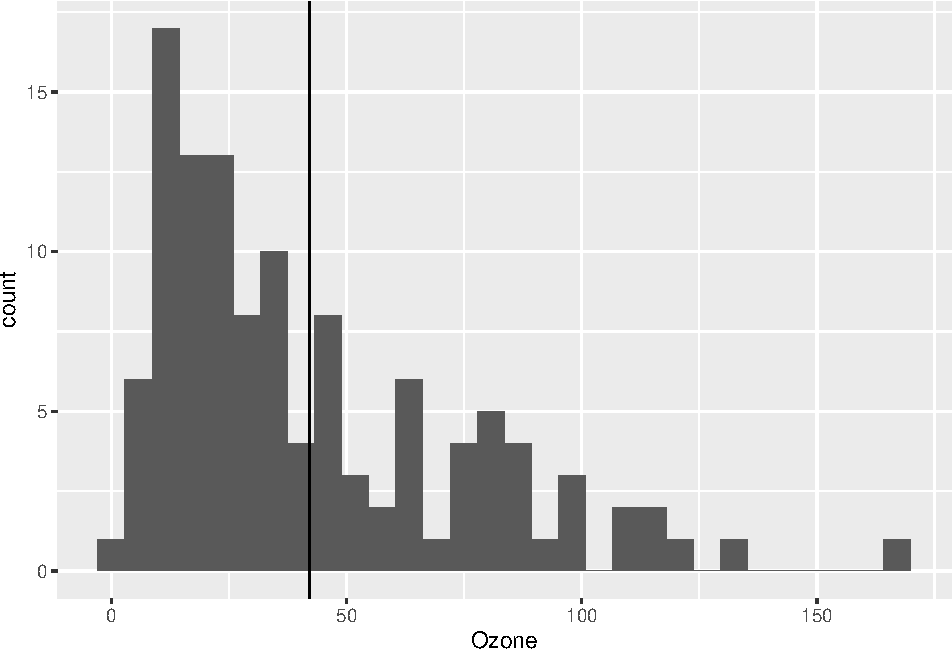
\includegraphics[width=0.5\linewidth]{manuscript_files/figure-latex/unnamed-chunk-3-1} \end{center}

Implementing with students may require a discussion about dollar sign
syntax and how geom\_vline is actually a special geom -- an annotation
-- rather than being mapped to the data. None of this is relevant to the
point you as a \emph{statistics} instructor aim to make: that the the
mean is the balancing point of the data or maybe a comment about
skewness.

Further, for the case of adding a vertical line at the mean for
different subsets of the data, a different approach is required. This
enterprise may take instructor/analyst/student on an even larger detour
-- possibly searching the internet, and maybe landing on the following
stack overflow page where 11,000 analytics searchers have landed:

\url{https://stackoverflow.com/questions/1644661/add-a-vertical-line-with-different-intercept-for-each-panel-in-ggplot2}

The solutions to this problem involve data manipulation \emph{prior} to
plotting the data. The solution disrupts the forward flow ggplot build.
One must take a pause, which may involve toggling back and forth between
stack overflow solutions, disrupting momentum you are working on to talk
about the pooled mean and the conditional mean.

``Learning becomes less efficient as the mental load students must carry
increases.'' \citep{lovett2000statscongnitive}

\begin{Shaded}
\begin{Highlighting}[]
\NormalTok{airquality }\OperatorTok\StringTok{ }
\StringTok{  }\KeywordTok{group_by}\NormalTok{(Month) }\OperatorTok\StringTok{ }
\StringTok{  }\KeywordTok{summarise}\NormalTok{(}\DataTypeTok{Ozone_mean =} \KeywordTok{mean}\NormalTok{(Ozone, }\DataTypeTok{na.rm =}\NormalTok{ T)) ->}
\NormalTok{airquality_by_month}

\KeywordTok{ggplot}\NormalTok{(airquality) }\OperatorTok{+}\StringTok{ }
\StringTok{  }\KeywordTok{aes}\NormalTok{(}\DataTypeTok{x =}\NormalTok{ Ozone) }\OperatorTok{+}\StringTok{ }
\StringTok{  }\KeywordTok{geom_histogram}\NormalTok{() }\OperatorTok{+}\StringTok{ }
\StringTok{  }\KeywordTok{facet_grid}\NormalTok{(}\DataTypeTok{rows =} \KeywordTok{vars}\NormalTok{(Month)) }\OperatorTok{+}
\StringTok{  }\KeywordTok{geom_vline}\NormalTok{(}\DataTypeTok{data =}\NormalTok{ airquality_by_month, }
             \KeywordTok{aes}\NormalTok{(}\DataTypeTok{xintercept =} 
\NormalTok{               Ozone_mean))}
\end{Highlighting}
\end{Shaded}

\begin{center}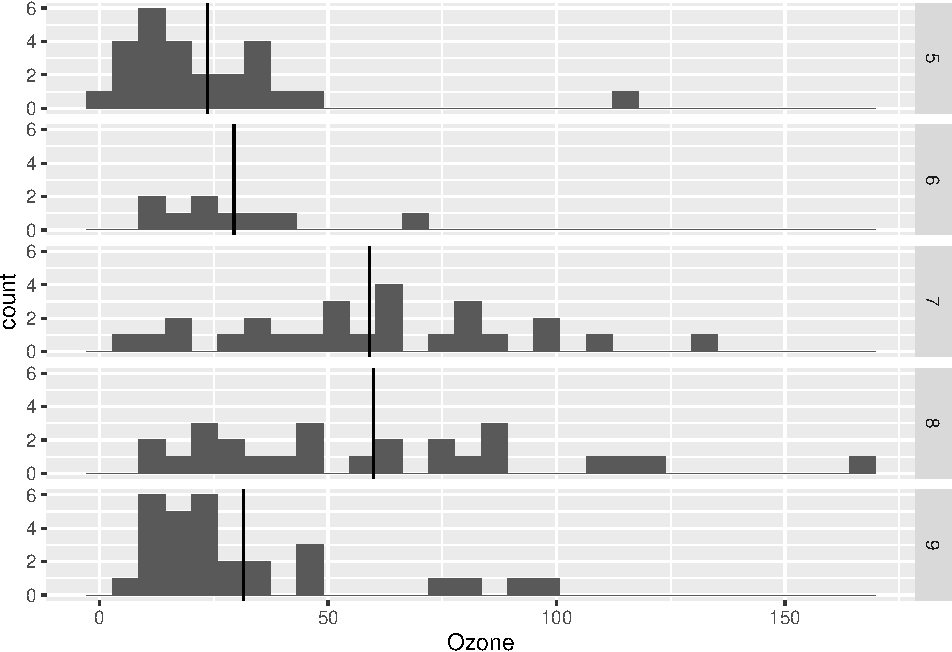
\includegraphics[width=0.5\linewidth]{manuscript_files/figure-latex/unnamed-chunk-4-1} \end{center}

\hypertarget{the-promise}{%
\subsection{The promise}\label{the-promise}}

But, using statistical geometries in ggplot2 \emph{can} feel simple.
geom\_smooth() adds loess fit of data to visualizations in an effortless
way; and an ordinary least squares fit is added almost as easily. And
geom\_boxplot reveals a 5-statistic summary of data medians, the inner
quartile range and min/max values in a single call. The popularity of
these easy-to-use functions is evident. geom\_smooth is used more than
82,000 times in .R and .Rmd files on GitHub and geom\_boxplot 93,000
times in .R and .Rmd files.

With these geoms one says ``let there be boxplots'' and there are
boxplots, and ``let there be loess smoothing'' and there is loess
smoothing. The same powerful, declarative experience can be arranged for
more statistical concepts.

\hypertarget{why-some-statistical-geoms-exist-and-others-dont}{%
\subsection{Why some statistical geoms exist and others
don't}\label{why-some-statistical-geoms-exist-and-others-dont}}

ggplot2 developers and maintainers, with the aim of keeping the code
base robust and reliable, have intentionally limited the out-of-the-box
geoms (as well as other variants) delivered in base ggplot2.

\begin{quote}
``ggplot2 is already pretty big \ldots{} and it's simply not feasible
for us to include all visualization possibilities into ggplot2 itself.''
- Thomas Pederson
\url{https://www.rstudio.com/resources/rstudioconf-2020/extending-your-ability-to-extend-ggplot2/}
\end{quote}

The ggplot2 extension system is designed to allow for more possibilities
and additional statistical vocabulary.

\begin{quote}
``It's much better to \ldots{} spread it out on multiple maintainers,
multiple specific packages and so on.''
\end{quote}

Extending ggplot statistical geometries will allow teachers, analysts
and students the ease of visual representation for a large number of
other desirable statistical summaries as is experienced with `base'
ggplot2 functions geom\_boxplot and geom\_smooth.

\hypertarget{introducing-ggxmean}{%
\subsection{introducing \{ggxmean\}}\label{introducing-ggxmean}}

The development package ggxmean
(\url{https://github.com/EvaMaeRey/ggxmean}) is aimed at providing more
statistical geometries that are practical for statistical educators and
analysts alike.

First, I present the geom\_x\_mean() function, which can be used in
place of the above solutions to drawing a vertical line at the mean at x
or the conditional mean of x. Note: functions from the development
package package are indicated with a comment.

The function geom\_x\_mean is used in a declarative way. After building
a plot showing the distribution of parts per billion of ozone in NYC,
you can add a vertical line at the mean with geom\_x\_mean(). The mean
is computed for the user automatically in the background.

Additionally, the conditional means are computed based on grouping
variables with geom\_x\_mean. Below, a second version of the plot is
also produced, where the mean of x computed for subsets of the data --
faceting by month. The group-wise computational of each mean is managed
in the background by the geom\_x\_mean function.

\begin{Shaded}
\begin{Highlighting}[]
\KeywordTok{library}\NormalTok{(ggplot2)}
\KeywordTok{library}\NormalTok{(ggxmean)}
\KeywordTok{ggplot}\NormalTok{(airquality) }\OperatorTok{+}\StringTok{ }
\StringTok{  }\KeywordTok{aes}\NormalTok{(}\DataTypeTok{x =}\NormalTok{ Ozone) }\OperatorTok{+}\StringTok{ }
\StringTok{  }\KeywordTok{geom_histogram}\NormalTok{() }\OperatorTok{+}\StringTok{ }
\StringTok{  }\KeywordTok{geom_x_mean}\NormalTok{() }\CommentTok{# ggxmean}
\end{Highlighting}
\end{Shaded}

\begin{Shaded}
\begin{Highlighting}[]
\KeywordTok{last_plot}\NormalTok{() }\OperatorTok{+}\StringTok{ }
\StringTok{  }\KeywordTok{facet_grid}\NormalTok{(}\DataTypeTok{rows =} \KeywordTok{vars}\NormalTok{(Month))}
\end{Highlighting}
\end{Shaded}

\hypertarget{other-statistical-geometries-in-the-ggxmean-package}{%
\subsection{Other statistical geometries in the \{ggxmean\}
package}\label{other-statistical-geometries-in-the-ggxmean-package}}

Beyond providing an easy way to add vertical line at the mean -- and
conditional means, \{ggxmean\} provides a number of other handy
geometries.

\hypertarget{other-univariate-markers}{%
\subsubsection{Other univariate
markers}\label{other-univariate-markers}}

\begin{Shaded}
\begin{Highlighting}[]
\KeywordTok{ggplot}\NormalTok{(airquality) }\OperatorTok{+}\StringTok{ }
\StringTok{  }\KeywordTok{aes}\NormalTok{(}\DataTypeTok{x =}\NormalTok{ Ozone) }\OperatorTok{+}\StringTok{ }
\StringTok{  }\KeywordTok{geom_histogram}\NormalTok{() }\OperatorTok{+}\StringTok{ }
\StringTok{  }\KeywordTok{geom_x_median}\NormalTok{() }\OperatorTok{+}\StringTok{ }
\StringTok{  }\KeywordTok{geom_x_quantile}\NormalTok{(}\DataTypeTok{quantile =} \FloatTok{.25}\NormalTok{,}
                  \DataTypeTok{linetype =} \StringTok{"dashed"}\NormalTok{) }\OperatorTok{+}\StringTok{ }
\StringTok{  }\KeywordTok{geom_x_percentile}\NormalTok{(}\DataTypeTok{percentile =} \DecValTok{100}\NormalTok{,}
                    \DataTypeTok{linetype =} \StringTok{"dotted"}\NormalTok{)}
\end{Highlighting}
\end{Shaded}

\begin{center}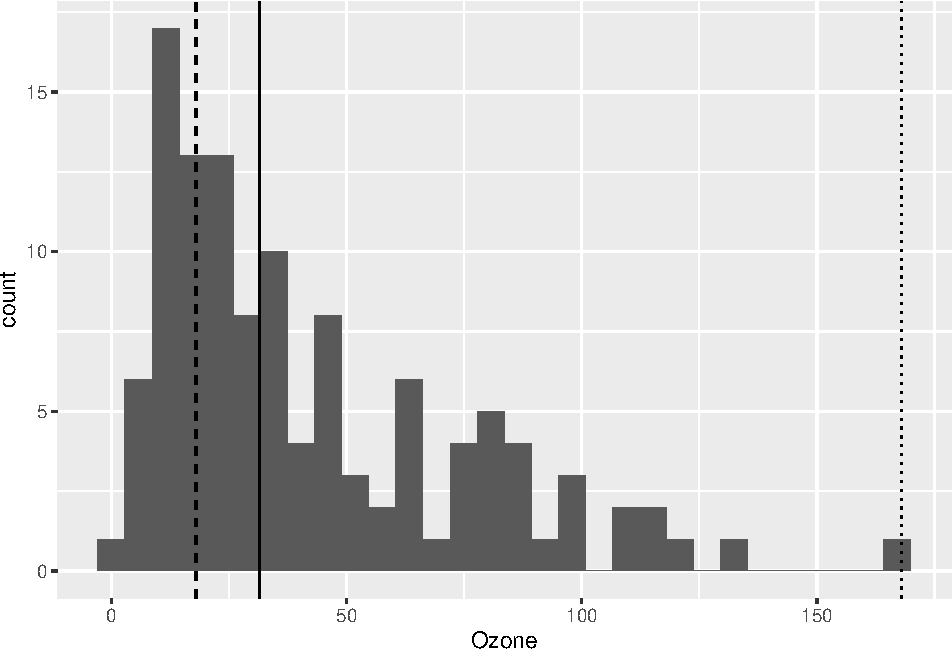
\includegraphics[width=0.5\linewidth]{manuscript_files/figure-latex/unnamed-chunk-6-1} \end{center}

All of these markers inherit from a new geom: geom\_xline(), which
unlink geom\_vline() is not an annotation layer, but rather can
represent a variable of the declared data set to the x position on the
plot.

\hypertarget{related-to-the-linear-model}{%
\subsubsection{Related to the linear
model}\label{related-to-the-linear-model}}

\begin{Shaded}
\begin{Highlighting}[]
\KeywordTok{ggplot}\NormalTok{(}\DataTypeTok{data =}\NormalTok{ cars) }\OperatorTok{+}\StringTok{ }
\StringTok{  }\KeywordTok{aes}\NormalTok{(speed, dist) }\OperatorTok{+}\StringTok{ }
\StringTok{  }\KeywordTok{geom_point}\NormalTok{() }\OperatorTok{+}\StringTok{ }\CommentTok{#BREAK}
\StringTok{  }\NormalTok{ggxmean}\OperatorTok{::}\KeywordTok{geom_lm}\NormalTok{() }\OperatorTok{+}\StringTok{ }\CommentTok{#BREAK}
\StringTok{  }\NormalTok{ggxmean}\OperatorTok{::}\KeywordTok{geom_lm_fitted}\NormalTok{(}\DataTypeTok{color =} \StringTok{"blue"}\NormalTok{,}
                          \DataTypeTok{size =} \DecValTok{3}\NormalTok{) }\OperatorTok{+}\StringTok{ }\CommentTok{#BREAK}
\StringTok{  }\NormalTok{ggxmean}\OperatorTok{::}\KeywordTok{geom_lm_residuals}\NormalTok{() }\OperatorTok{+}\StringTok{ }\CommentTok{#BREAK}
\StringTok{  }\NormalTok{ggxmean}\OperatorTok{::}\KeywordTok{geom_lm_conf_int}\NormalTok{() }\OperatorTok{+}\StringTok{ }\CommentTok{#BREAK}
\StringTok{  }\NormalTok{ggxmean}\OperatorTok{::}\KeywordTok{geom_lm_intercept}\NormalTok{(}\DataTypeTok{color =} \StringTok{"red"}\NormalTok{,}
                             \DataTypeTok{size =} \DecValTok{5}\NormalTok{) }\OperatorTok{+}\StringTok{ }\CommentTok{#BREAK}
\StringTok{  }\NormalTok{ggxmean}\OperatorTok{::}\KeywordTok{geom_lm_formula}\NormalTok{(}\DataTypeTok{size =} \DecValTok{10}\NormalTok{) }\CommentTok{#BREAK}
\end{Highlighting}
\end{Shaded}

\begin{center}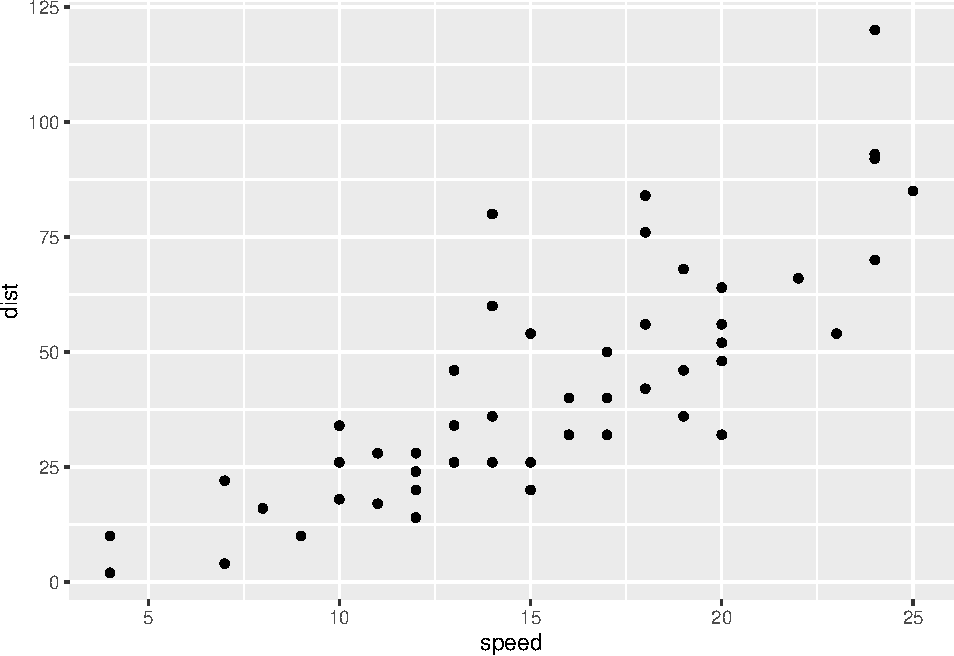
\includegraphics[width=0.3\linewidth]{manuscript_files/figure-latex/unnamed-chunk-7-1} 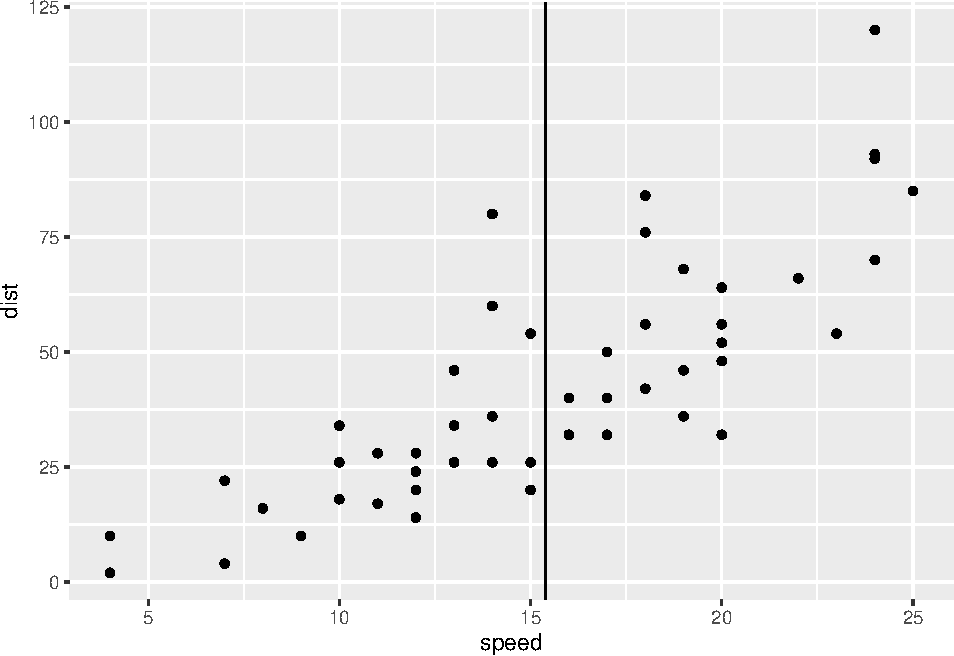
\includegraphics[width=0.3\linewidth]{manuscript_files/figure-latex/unnamed-chunk-7-2} \end{center}

\hypertarget{related-to-covariance}{%
\subsubsection{Related to covariance}\label{related-to-covariance}}

\emph{return to this section}

\begin{Shaded}
\begin{Highlighting}[]
\KeywordTok{ggplot}\NormalTok{(}\DataTypeTok{data =}\NormalTok{ cars) }\OperatorTok{+}\StringTok{ }
\StringTok{  }\KeywordTok{aes}\NormalTok{(speed, dist) }\OperatorTok{+}\StringTok{ }
\StringTok{  }\KeywordTok{geom_point}\NormalTok{() }\OperatorTok{+}\StringTok{ }\CommentTok{#BREAK}
\StringTok{  }\KeywordTok{geom_x_mean}\NormalTok{()}
\end{Highlighting}
\end{Shaded}

\hypertarget{fitting-distributions}{%
\subsubsection{fitting distributions}\label{fitting-distributions}}

\begin{Shaded}
\begin{Highlighting}[]
\KeywordTok{ggplot}\NormalTok{(}\DataTypeTok{data =}\NormalTok{ faithful) }\OperatorTok{+}\StringTok{ }
\StringTok{  }\KeywordTok{aes}\NormalTok{(waiting) }\OperatorTok{+}\StringTok{ }
\StringTok{  }\KeywordTok{geom_rug}\NormalTok{() }\OperatorTok{+}\StringTok{ }
\StringTok{  }\KeywordTok{geom_histogram}\NormalTok{(}\KeywordTok{aes}\NormalTok{(}\DataTypeTok{y =}\NormalTok{ ..density..)) }\OperatorTok{+}\StringTok{ }\CommentTok{#BREAK}
\StringTok{  }\NormalTok{ggxmean}\OperatorTok{::}\KeywordTok{geom_normal_dist}\NormalTok{(}\DataTypeTok{fill =} \StringTok{"blue"}\NormalTok{) }\OperatorTok{+}\StringTok{ }\CommentTok{#BREAK}
\StringTok{  }\KeywordTok{facet_grid}\NormalTok{(}\DataTypeTok{rows =} \KeywordTok{vars}\NormalTok{(eruptions }\OperatorTok{>}\StringTok{ }\DecValTok{3}\NormalTok{)) }\CommentTok{#BREAK}
\end{Highlighting}
\end{Shaded}

\begin{center}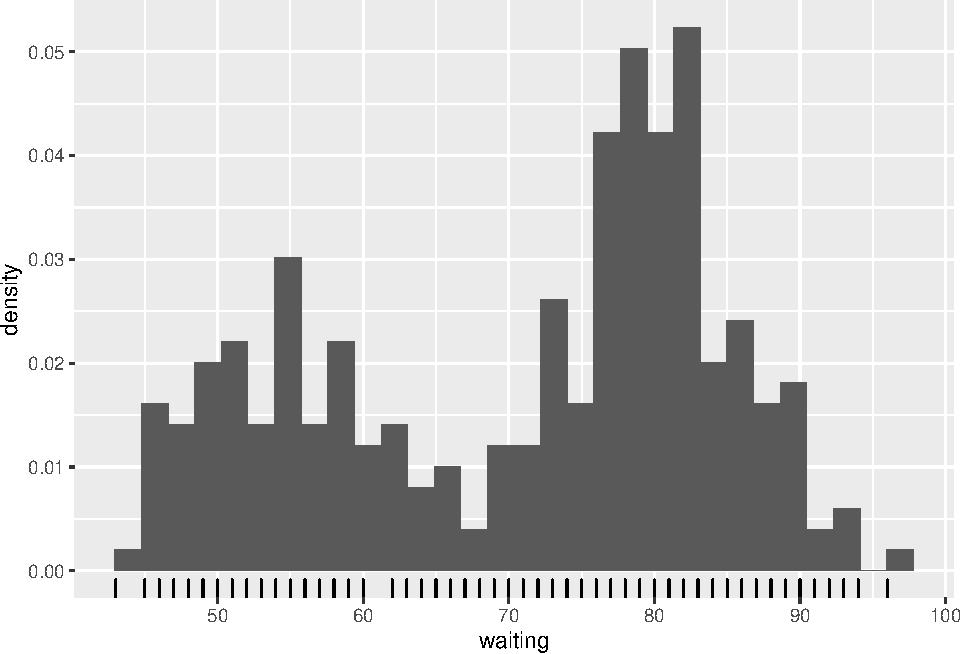
\includegraphics[width=0.3\linewidth]{manuscript_files/figure-latex/unnamed-chunk-8-1} 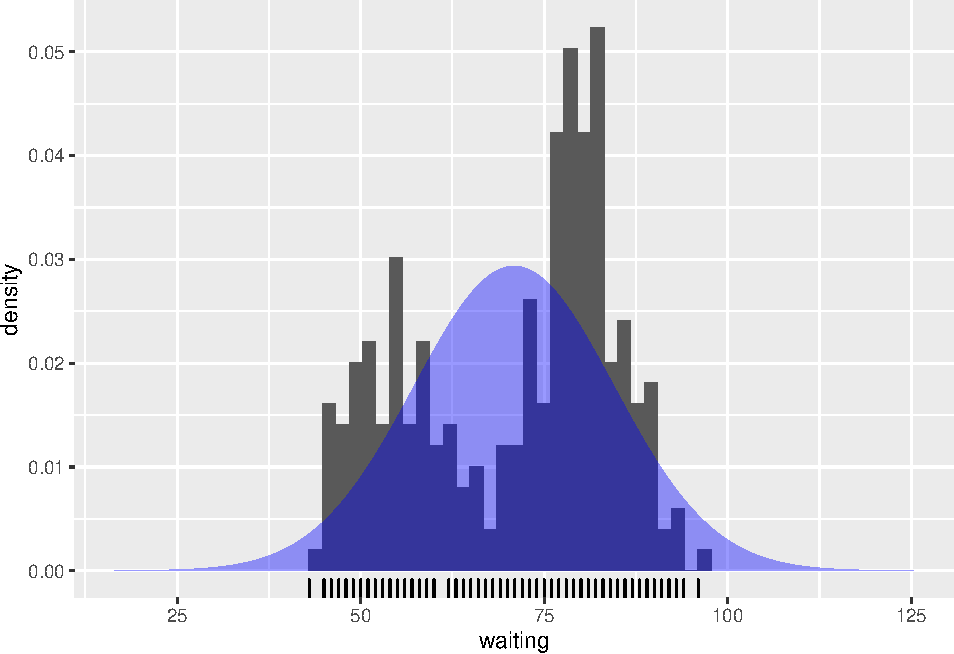
\includegraphics[width=0.3\linewidth]{manuscript_files/figure-latex/unnamed-chunk-8-2} 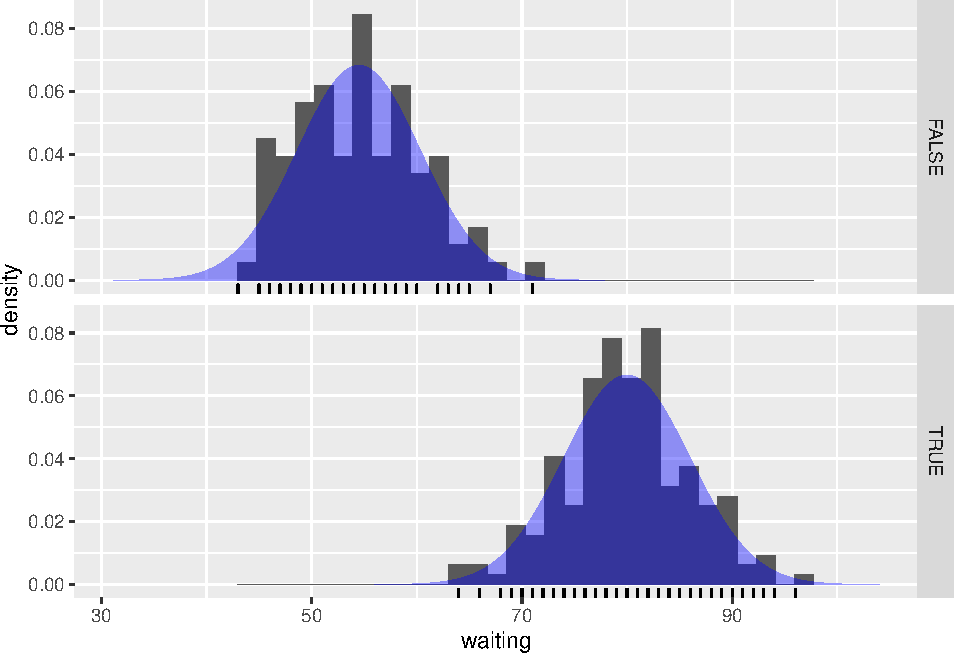
\includegraphics[width=0.3\linewidth]{manuscript_files/figure-latex/unnamed-chunk-8-3} \end{center}

\hypertarget{annotation-stamps}{%
\subsection{Annotation: Stamps}\label{annotation-stamps}}

\begin{Shaded}
\begin{Highlighting}[]
\KeywordTok{library}\NormalTok{(patchwork)}
\NormalTok{(}\KeywordTok{ggplot}\NormalTok{(}\DataTypeTok{data =}\NormalTok{ cars) }\OperatorTok{+}
\StringTok{  }\KeywordTok{aes}\NormalTok{(dist) }\OperatorTok{+}
\StringTok{  }\NormalTok{ggxmean}\OperatorTok{::}\KeywordTok{stamp_normal_dist}\NormalTok{() ) }\OperatorTok{/}
\NormalTok{(}\KeywordTok{ggplot}\NormalTok{(}\DataTypeTok{data =}\NormalTok{ cars) }\OperatorTok{+}
\StringTok{  }\KeywordTok{aes}\NormalTok{(dist) }\OperatorTok{+}
\StringTok{  }\NormalTok{ggxmean}\OperatorTok{::}\KeywordTok{stamp_normal_prob}\NormalTok{())}
\end{Highlighting}
\end{Shaded}

\begin{center}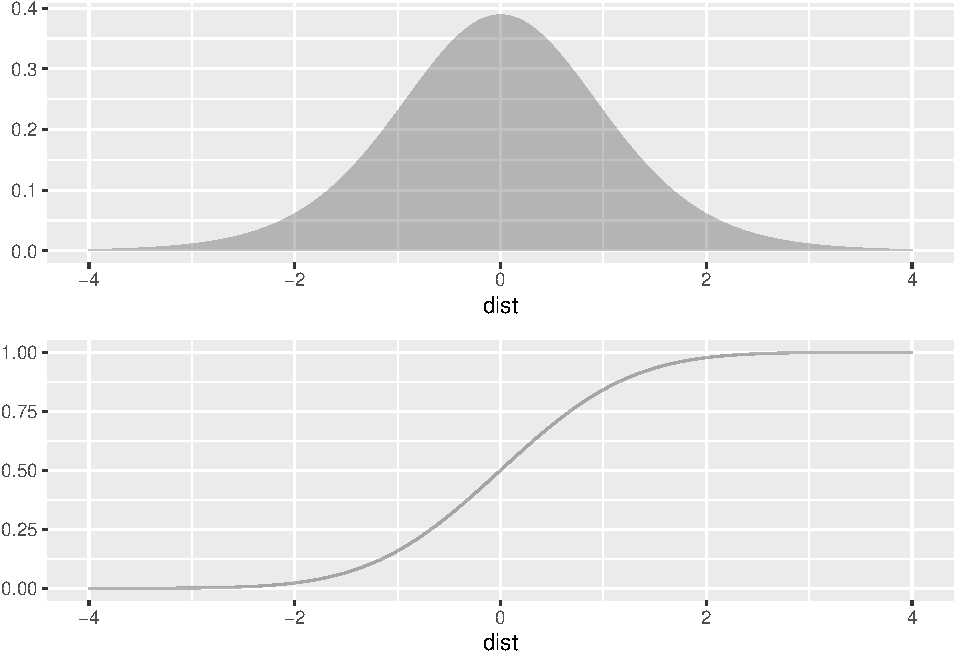
\includegraphics[width=0.5\linewidth]{manuscript_files/figure-latex/unnamed-chunk-9-1} \end{center}

\begin{Shaded}
\begin{Highlighting}[]
\KeywordTok{ggplot}\NormalTok{(cars, }\KeywordTok{aes}\NormalTok{(}\DataTypeTok{x =}\NormalTok{ speed)) }\OperatorTok{+}
\StringTok{  }\KeywordTok{geom_rug}\NormalTok{(}\DataTypeTok{alpha =} \FloatTok{.3}\NormalTok{) }\OperatorTok{+}
\StringTok{  }\KeywordTok{geom_normal_dist}\NormalTok{() }\OperatorTok{+}\StringTok{ }
\StringTok{  }\KeywordTok{stamp_normal_dist}\NormalTok{()}
\end{Highlighting}
\end{Shaded}

\begin{center}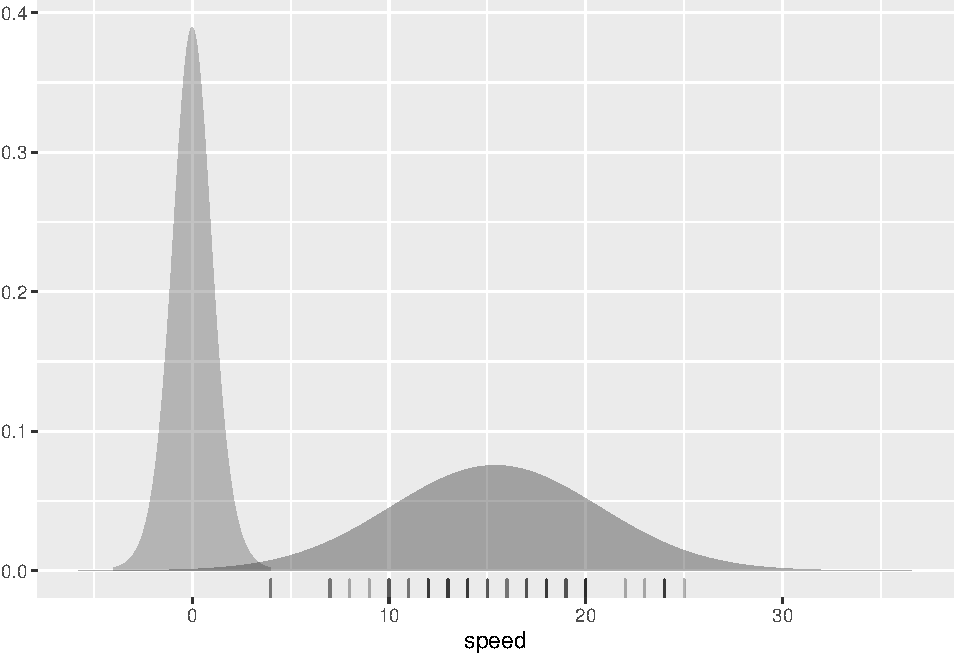
\includegraphics[width=0.5\linewidth]{manuscript_files/figure-latex/unnamed-chunk-10-1} \end{center}

\hypertarget{stamp-space}{%
\subsubsection{stamp space?}\label{stamp-space}}

\begin{Shaded}
\begin{Highlighting}[]
\NormalTok{ggxmean}\OperatorTok{:::}\KeywordTok{stamp_space}\NormalTok{() }\OperatorTok{+}
\StringTok{  }\KeywordTok{stamp_normal_dist}\NormalTok{(}\DataTypeTok{fill =} \StringTok{"steelblue"}\NormalTok{)}
\end{Highlighting}
\end{Shaded}

\begin{center}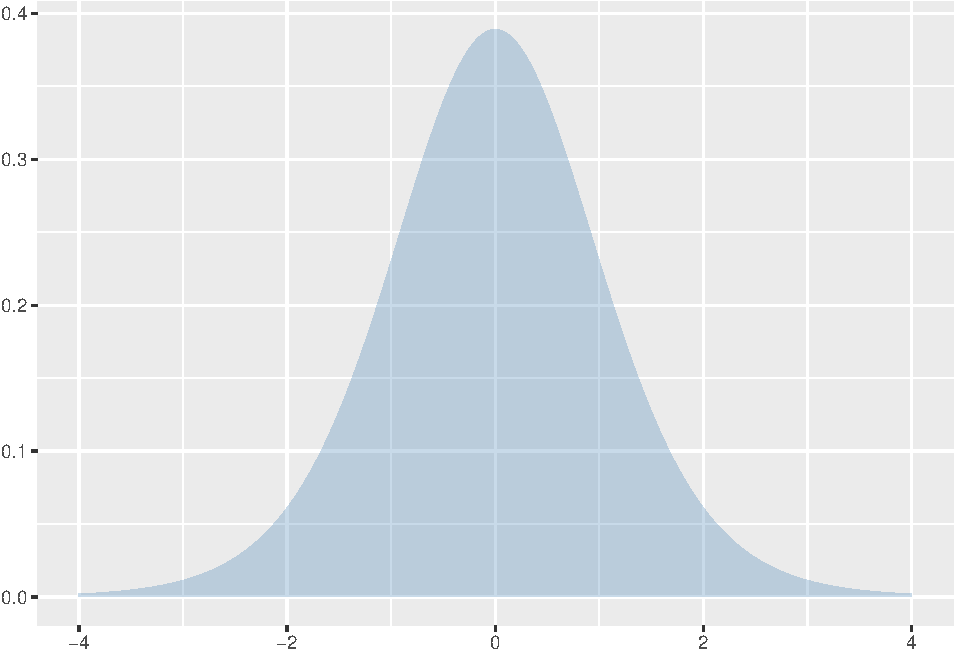
\includegraphics[width=0.5\linewidth]{manuscript_files/figure-latex/unnamed-chunk-11-1} \end{center}

\begin{Shaded}
\begin{Highlighting}[]
\KeywordTok{last_plot}\NormalTok{() }\OperatorTok{+}
\StringTok{  }\KeywordTok{stamp_t_dist}\NormalTok{(}\DataTypeTok{df =} \DecValTok{3}\NormalTok{, }
               \DataTypeTok{fill =} \StringTok{"goldenrod"}\NormalTok{,}
               \DataTypeTok{linetype =} \StringTok{"dashed"}\NormalTok{,}
               \DataTypeTok{color =} \StringTok{"goldenrod"}\NormalTok{,}
               \DataTypeTok{outline.type =} \StringTok{"upper"}\NormalTok{)}
\end{Highlighting}
\end{Shaded}

\begin{center}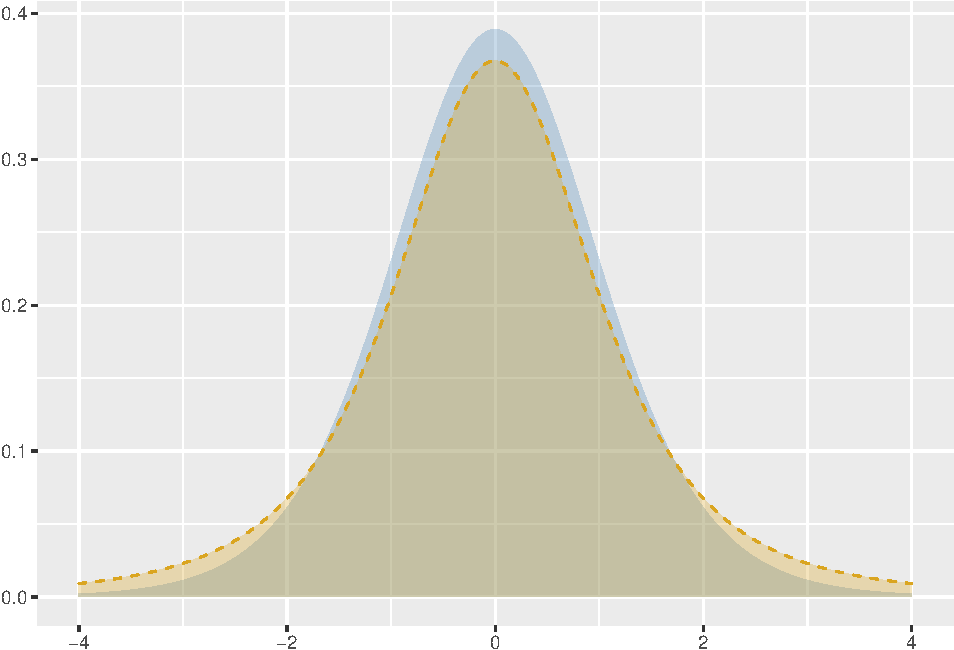
\includegraphics[width=0.5\linewidth]{manuscript_files/figure-latex/unnamed-chunk-11-2} \end{center}

\begin{Shaded}
\begin{Highlighting}[]
\KeywordTok{library}\NormalTok{(patchwork)}
\KeywordTok{library}\NormalTok{(ggplot2)}
\KeywordTok{library}\NormalTok{(ggxmean)}
\NormalTok{ggxmean}\OperatorTok{:::}\KeywordTok{stamp_space}\NormalTok{() }\OperatorTok{+}
\StringTok{  }\KeywordTok{stamp_normal_dist}\NormalTok{()}

\NormalTok{ggxmean}\OperatorTok{:::}\KeywordTok{stamp_space}\NormalTok{() }\OperatorTok{+}
\StringTok{  }\KeywordTok{stamp_chi_dist}\NormalTok{() }\OperatorTok{+}\StringTok{ }
\StringTok{  }\KeywordTok{stamp_t_dist}\NormalTok{()}

\NormalTok{ggxmean}\OperatorTok{:::}\KeywordTok{stamp_space}\NormalTok{() }\OperatorTok{+}
\StringTok{  }\NormalTok{ggxmean}\OperatorTok{::}\KeywordTok{stamp_normal_dist}\NormalTok{(}\DataTypeTok{x_min =} \DecValTok{-1}\NormalTok{, }\DataTypeTok{x_max =} \DecValTok{1}\NormalTok{, }\DataTypeTok{color =} \StringTok{"black"}\NormalTok{, }\DataTypeTok{outline.type =} \StringTok{"full"}\NormalTok{) }\OperatorTok{+}
\StringTok{  }\NormalTok{ggxmean}\OperatorTok{::}\KeywordTok{stamp_normal_dist}\NormalTok{(}\DataTypeTok{x_min =} \DecValTok{-2}\NormalTok{, }\DataTypeTok{x_max =} \DecValTok{2}\NormalTok{, }\DataTypeTok{color =} \StringTok{"black"}\NormalTok{, }\DataTypeTok{outline.type =} \StringTok{"full"}\NormalTok{) }\OperatorTok{+}
\StringTok{  }\NormalTok{ggxmean}\OperatorTok{::}\KeywordTok{stamp_normal_dist}\NormalTok{(}\DataTypeTok{x_min =} \DecValTok{-3}\NormalTok{, }\DataTypeTok{x_max =} \DecValTok{3}\NormalTok{, }\DataTypeTok{color =} \StringTok{"black"}\NormalTok{, }\DataTypeTok{outline.type =} \StringTok{"full"}\NormalTok{) }\OperatorTok{+}
\StringTok{  }\NormalTok{ggxmean}\OperatorTok{::}\KeywordTok{stamp_normal_dist}\NormalTok{(}\DataTypeTok{x_min =} \DecValTok{-4}\NormalTok{, }\DataTypeTok{x_max =} \DecValTok{4}\NormalTok{, }\DataTypeTok{color =} \StringTok{"black"}\NormalTok{, }\DataTypeTok{outline.type =} \StringTok{"full"}\NormalTok{) }\OperatorTok{+}
\StringTok{  }\NormalTok{ggxmean}\OperatorTok{::}\KeywordTok{stamp_normal_dist}\NormalTok{(}\DataTypeTok{x_min =} \DecValTok{-5}\NormalTok{, }\DataTypeTok{x_max =} \DecValTok{5}\NormalTok{, }\DataTypeTok{color =} \StringTok{"black"}\NormalTok{, }\DataTypeTok{outline.type =} \StringTok{"full"}\NormalTok{) }\OperatorTok{+}
\StringTok{  }\KeywordTok{theme_minimal}\NormalTok{()}
\end{Highlighting}
\end{Shaded}

\begin{Shaded}
\begin{Highlighting}[]
\KeywordTok{library}\NormalTok{(patchwork)}

\NormalTok{ggxmean}\OperatorTok{:::}\KeywordTok{stamp_space}\NormalTok{() }\OperatorTok{+}
\StringTok{  }\KeywordTok{stamp_normal_dist}\NormalTok{(}\DataTypeTok{alpha =} \FloatTok{.05}\NormalTok{) }\OperatorTok{+}
\StringTok{  }\KeywordTok{stamp_normal_dist}\NormalTok{(}\DataTypeTok{x_min =} \DecValTok{-1}\NormalTok{, }\DataTypeTok{x_max =} \DecValTok{1}\NormalTok{) ->}
\NormalTok{p1}
    
\NormalTok{  ggxmean}\OperatorTok{:::}\KeywordTok{stamp_space}\NormalTok{() }\OperatorTok{+}
\StringTok{  }\KeywordTok{stamp_normal_prob}\NormalTok{(}\DataTypeTok{alpha =} \FloatTok{.1}\NormalTok{) }\OperatorTok{+}
\StringTok{  }\KeywordTok{stamp_normal_prob}\NormalTok{(}\DataTypeTok{sd_min =} \DecValTok{-1}\NormalTok{, }\DataTypeTok{sd_max =} \DecValTok{1}\NormalTok{, }
                             \DataTypeTok{size =} \FloatTok{1.5}\NormalTok{) ->}
\NormalTok{p2}
  
\NormalTok{p1 }\OperatorTok{/}\StringTok{ }\NormalTok{p2}
\end{Highlighting}
\end{Shaded}

\begin{center}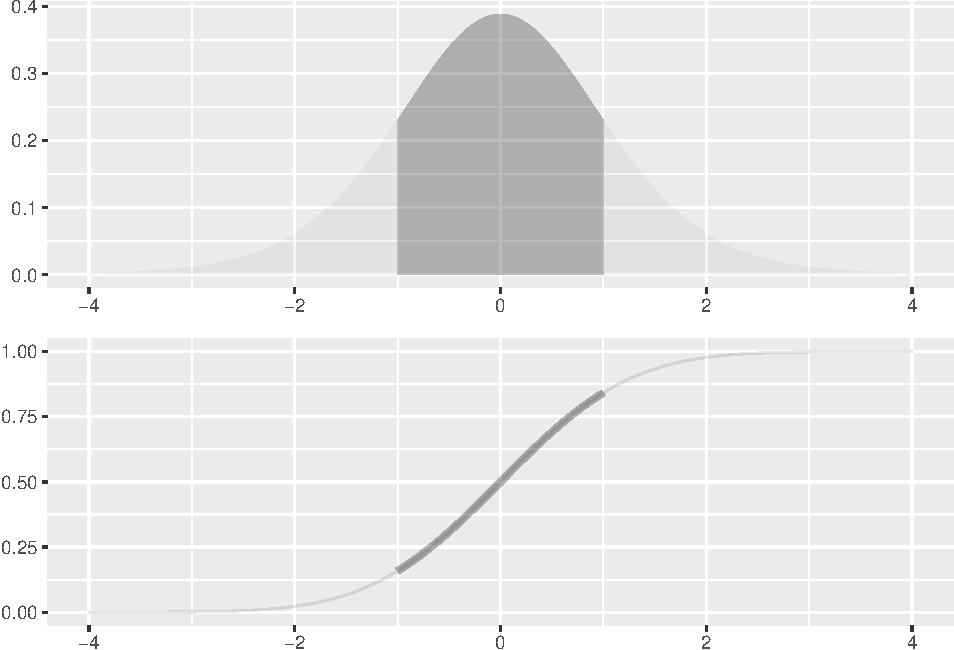
\includegraphics[width=0.5\linewidth]{manuscript_files/figure-latex/unnamed-chunk-13-1} \end{center}

\begin{Shaded}
\begin{Highlighting}[]
\KeywordTok{library}\NormalTok{(patchwork)}

\NormalTok{ggxmean}\OperatorTok{:::}\KeywordTok{stamp_space}\NormalTok{() }\OperatorTok{+}
\StringTok{  }\KeywordTok{stamp_chisq_dist}\NormalTok{(}\DataTypeTok{df =} \DecValTok{3}\NormalTok{,  }\DataTypeTok{fill =} \StringTok{"steelblue"}\NormalTok{) }\OperatorTok{+}
\StringTok{  }\KeywordTok{stamp_chisq_dist}\NormalTok{(}\DataTypeTok{df =} \DecValTok{5}\NormalTok{,  }\DataTypeTok{fill =} \StringTok{"goldenrod"}\NormalTok{) }\OperatorTok{+}
\StringTok{  }\KeywordTok{stamp_chisq_dist}\NormalTok{(}\DataTypeTok{df =} \DecValTok{7}\NormalTok{,  }\DataTypeTok{fill =} \StringTok{"plum"}\NormalTok{) }\OperatorTok{+}
\StringTok{  }\KeywordTok{stamp_chisq_dist}\NormalTok{(}\DataTypeTok{df =} \DecValTok{11}\NormalTok{, }\DataTypeTok{fill =} \StringTok{"sienna"}\NormalTok{) ->}
\NormalTok{g1}
  
\NormalTok{ggxmean}\OperatorTok{:::}\KeywordTok{stamp_space}\NormalTok{() }\OperatorTok{+}
\StringTok{  }\KeywordTok{stamp_chisq_prob}\NormalTok{(}\DataTypeTok{df =} \DecValTok{3}\NormalTok{,  }\DataTypeTok{color =} \StringTok{"steelblue"}\NormalTok{) }\OperatorTok{+}
\StringTok{  }\KeywordTok{stamp_chisq_prob}\NormalTok{(}\DataTypeTok{df =} \DecValTok{5}\NormalTok{,  }\DataTypeTok{color =} \StringTok{"goldenrod"}\NormalTok{) }\OperatorTok{+}
\StringTok{  }\KeywordTok{stamp_chisq_prob}\NormalTok{(}\DataTypeTok{df =} \DecValTok{7}\NormalTok{,  }\DataTypeTok{color =} \StringTok{"plum"}\NormalTok{) }\OperatorTok{+}
\StringTok{  }\KeywordTok{stamp_chisq_prob}\NormalTok{(}\DataTypeTok{df =} \DecValTok{11}\NormalTok{, }\DataTypeTok{color =} \StringTok{"sienna"}\NormalTok{) ->}
\NormalTok{g2}

\NormalTok{g1 }\OperatorTok{/}\StringTok{ }\NormalTok{g2}
\end{Highlighting}
\end{Shaded}

\begin{center}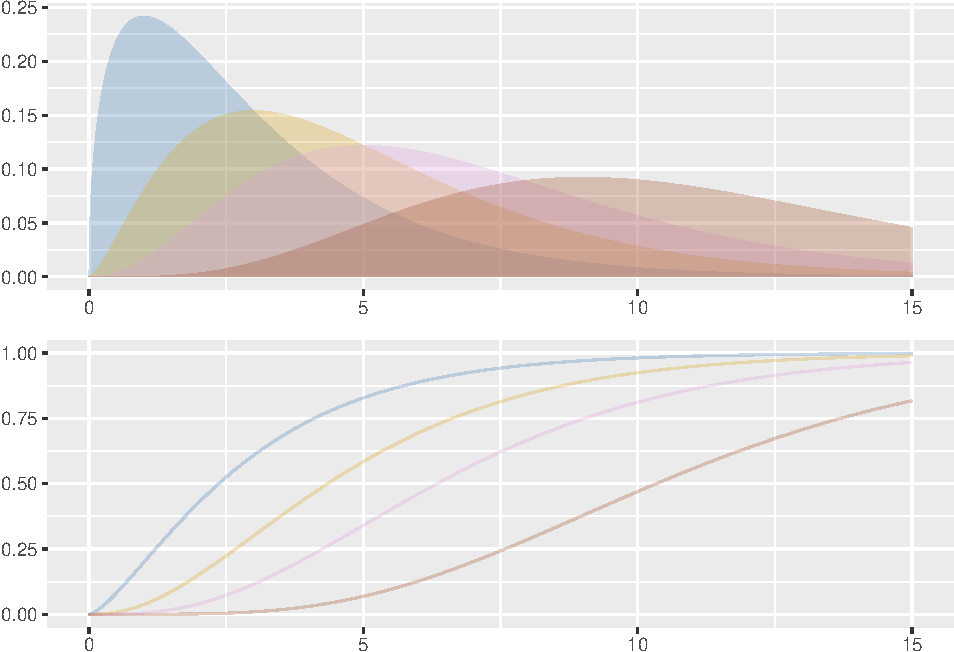
\includegraphics[width=0.5\linewidth]{manuscript_files/figure-latex/unnamed-chunk-14-1} \end{center}

\citep{tishkovskaya2012statistical}

\bibliographystyle{agsm}
\bibliography{bibliography.bib}

\end{document}
